\section*{Lecture 22}

\subsection*{1.} Let $\Vec{a} = \left( 1,1,1 \right) $ and $\Vec{b} = \left( 1,2,1 \right) $. Find $\Vec{a} \times \Vec{b}, \Vec{a} \times \left( \Vec{a} \times \Vec{b} \right) $ and $\left( \Vec{a} \times \Vec{b} \right) \times \left( \Vec{a} \times \Vec{b} \right)$.
\bigbreak
First we find $\Vec{a} \times \Vec{b}$ by the normal vector product formula:
\[ 
\Vec{a}\times \Vec{b} = \left| \begin{array}{ccc}
\Vec{i} & \Vec{j} & \Vec{k}\\
1 & 1 & 1\\
1 & 2 & 1\\
\end{array} \right| = \Vec{i} \left| \begin{array}{cc}
1 & 1\\
2 & 1\\
\end{array} \right| - \Vec{j} \left| \begin{array}{cc}
1 & 1\\
1 & 1\\
\end{array} \right| + \Vec{k} \left| \begin{array}{cc}
1 & 1\\
1 & 2\\
\end{array} \right| = \left( -1, 0, 1 \right) 
.\]
For $\Vec{a} \times \left( \Vec{a} \times \Vec{b} \right) $ we can use the fact that $\Vec{a} \times \Vec{b} = \left( -1, 0, 1 \right) $ and get:
\[ 
\Vec{a} \times \left( \Vec{a} \times \Vec{b} \right) = \left| \begin{array}{ccc}
\Vec{i} & \Vec{j} & \Vec{k}\\
1 & 1 & 1\\
-1 & 0 & 1\\
\end{array} \right| = \Vec{i} \left| \begin{array}{cc}
1 & 1\\
0 & 1\\
\end{array} \right| - \Vec{j} \left| \begin{array}{cc}
1 & 1\\
-1 & 1\\
\end{array} \right| + \Vec{k} \left| \begin{array}{cc}
1 & 1\\
-1 & 0\\
\end{array} \right| = \left( 1, -2, 1 \right) 
.\]
For $\left( \Vec{a}\times \Vec{b} \right) \times \left( \Vec{a} \times \Vec{b} \right) $ we can once again utilize that $\Vec{a} \times \Vec{b} = \left( -1, 0, 1 \right) $ and get:
\[ 
  \left( \Vec{a} \times \Vec{b} \right)  \times \left( \Vec{a} \times \Vec{b} \right) = \left| \begin{array}{ccc}
  \Vec{i} & \Vec{j} & \Vec{k}\\
  -1 & 0 & 1\\
  -1 & 0 & 1\\
  \end{array} \right| = \Vec{i} \left| \begin{array}{cc}
  0 & 1\\
  0 & 1\\
  \end{array} \right| - \Vec{j} \left| \begin{array}{cc}
  -1 & 1\\
  -1 & 1\\
  \end{array} \right| + \Vec{k} \left| \begin{array}{cc}
  -1 & 0\\
  -1 & 0\\
  \end{array} \right| = \left( 0, 0, 0 \right)
.\]



\subsection*{2.} Let
\[ 
\Vec{v} \left( x,y,z \right) = \left( v_1 \left( x,y,z \right), v_2 \left( x,y,z \right), v_3 \left( x,y,z \right)  \right) = \left( xyz, x \cos \left( yz \right) , z e^{xy} \right) 
.\]
Calculate
\[ 
\Vec{v}_x \left( x,y,z \right), \Vec{v}_y \left( x,y,z \right), \Vec{v}_z \left( x,y,z \right), \Vec{v}_{xy} \left( x,y,z \right)
\]
where
\[ 
\Vec{v}_{xy} \left( x,y,z \right) = \left( \frac{\partial^2}{\partial x \partial y} v_1 \left( x,y,z \right), \frac{\partial^2}{\partial x \partial y} v_2 \left( x,y,z \right), \frac{\partial^2}{\partial x \partial y} v_3 \left( x,y,z \right) \right) 
.\]
\bigbreak
First we find $\Vec{v}_x \left( x, y, z \right) $ by keeping $y$ and $z$ fixed whilst differentiating with respect to $x$ in $\Vec{v}$ as:
\[ 
\Vec{v}_x \left( x, y, z \right) = \left( yz, \cos \left( yz \right), zy e^{xy} \right) 
.\]
Now when differentiating with respect to $y$ to get $\Vec{v}_y$ we get:
\[ 
\Vec{v}_y \left( x,y, z \right) = \left( xz, -zx \sin \left( yz \right), xz e^{xy} \right) 
.\]
When differentiating with respect to $z$ to get $\Vec{v}_z$ we get:
\[ 
\Vec{v}_z \left( x, y, z \right) = \left( xy, -xy \sin \left( yz \right), e^{xy}  \right) 
.\]
When wanting to find $\Vec{v}_{xy} \left( x,y,z \right) $ we must differentiate $\Vec{v}_y$ with respect to $x$ as:
\[ 
\Vec{v}_{xy} = \frac{\mathrm{d}}{\mathrm{d}x} \Vec{v}_y = \left( z, -z \sin \left( yz \right) , z e^{xy} + zxy e^{xy} \right) 
.\]





\subsection*{3.} Consider the position vector $\Vec{r}(t) = \Vec{c} + t^2 \Vec{b}$ at time $t \geq 0$ of a moving particle where $\Vec{c} = \left( 1,1,0 \right) $ and $\Vec{b} = \left( 1,0,0 \right) $.

\paragraph{(a)} Sketch the path of the particle.
\bigbreak
\begin{figure}[ht]
    \centering
    \incfig[0.5]{e22f1}
    \caption{e22f1}
    \label{fig:e22f1}
\end{figure}

\paragraph{(b)} Calculate the velocity $\Vec{v}(t)$ and the acceleration $\Vec{a} (t)$.
\bigbreak
The velocity is simply the first derivative with respect to time which gives:
\[ 
\Vec{v}(t) = 2t \Vec{b}
.\]
The acceleration is the second derivative and thus:
\[ 
\Vec{a}(t) = 2\Vec{b}
.\]


\paragraph{(c)} Calculate the projection $p$ of $\Vec{a}(t)$ in direction of $\Vec{v}(t)$.
\bigbreak
The projection is calculated as:
\[ 
p = \frac{\Vec{a}(t) \cdot \Vec{v}(t)}{\left| \Vec{v}(t) \right|} = \frac{\left( 2,0,0 \right) \cdot \left( 2t, 0, 0 \right) }{\sqrt{\left( 2t \right) ^2}} = \frac{4t}{2t} = 2
.\]


\paragraph{(d)} The acceleration can be decomposed into a tangential acceleration $\Vec{a}_{\mathrm{tan}}(t)$ (in direction of $\Vec{v}(t)$) and a normal acceleration $\Vec{a}_{\mathrm{norm}}(t) $ (orthogonal to $\Vec{v}(t)$)
\[ 
\Vec{a}(t) = \Vec{a}_{\mathrm{tan}} (t) + \Vec{a}_{\mathrm{norm}}(t)
\]
where
\[ 
\Vec{a}_{\mathrm{tan}} (t) = p \frac{\Vec{v}(t)}{\left| \Vec{v}(t) \right|}
\]
and
\[ 
\Vec{a}_{\mathrm{norm}}(t) = \Vec{a}(t) - \Vec{a}_{\mathrm{tan}}(t)
.\]
Calculate $\Vec{a}_{\mathrm{tan}}(t)$ and $\Vec{a}_{\mathrm{norm}}(t)$.
\bigbreak
We can simply plug the values into the fomulae as:
\begin{align*}
  \Vec{a}_{\mathrm{tan}} (t) &= p \frac{\Vec{v}(t)}{\left| \Vec{v}(t) \right|} \\
  &= 2 \frac{\left( 2t,0,0 \right) }{2t} \\
  &= \left( 2,0,0 \right)  \\
  \Vec{a}_{\mathrm{norm}}(t) &= \Vec{a}(t) - \Vec{a}_{\mathrm{tan}}(t) \\
  &= \left( 2,0,0 \right) - \left( 2,0,0 \right)  \\
  &= (0,0,0)
.\end{align*}


\subsection*{4.} Consider the position vector $\Vec{r}(t) = \left( \cos t, \sin t, 0 \right) $ at time $t \geq 0$ of a moving particle.

\paragraph{(a)} Calculate the velocity $\Vec{v}(t)$ and the acceleration $\Vec{a}(t)$.
\bigbreak
The velocity is the first derivative and can be calculated as:
\[ 
\Vec{v}(t) = \left( -\sin t, \cos t, 0 \right)
.\]
The acceleration is the derivative of this (the second derivative) and can be calculated simply to be:
\[ 
\Vec{a}(t) = \left( -\cos t, -\sin t, 0 \right) 
.\]



\paragraph{(b)} Calculate the projection $p$ of $\Vec{a}(t)$ in direction of $\Vec{v}(t)$.
\bigbreak
We can simply use the projection formula again as:
\[ 
p = \frac{\Vec{a}(t) \cdot \Vec{v}(t)}{\left| \Vec{v}(t) \right|} = \frac{\left( -\cos t, -\sin t,0 \right) \cdot \left( -\sin t, \cos t,0 \right) }{\sqrt{\left( -\sin t \right)^2 + \left( \cos t \right)^2}} = \frac{\sin t \cos t - \sin t \cos t}{\sqrt{\left( - \sin t \right)^2 + \left( \cos t \right)^2}} = 0
.\]


\paragraph{(c)} Calculate $\Vec{a}_{\mathrm{tan}}(t)$ and $\Vec{a}_{\mathrm{norm}}(t)$.
\bigbreak
We can simply use the formulae again as:
\begin{align*}
  \Vec{a}_{\mathrm{tan}} &= p \frac{\Vec{v}(t)}{\left| \Vec{v}(t) \right|} \\
  &= 0 \\
  \Vec{a}_{\mathrm{norm}} &= \Vec{a}\left( t \right) - \Vec{a}_{\mathrm{tan}}(t) \\
  &= \Vec{a}(t) \\
  &= \left( -\cos t, - \sin t, 0 \right) 
.\end{align*}


\subsection*{5.} Consider the curve $C$ consisting of all points $P(x,y,z)$ such that
\[ 
  (x-1)^2 + (y-1)^2 = 1, \qquad z = 0
.\]

\paragraph{(a)} Sketch the curve $C$.
\begin{figure} [ht]
  \centering
  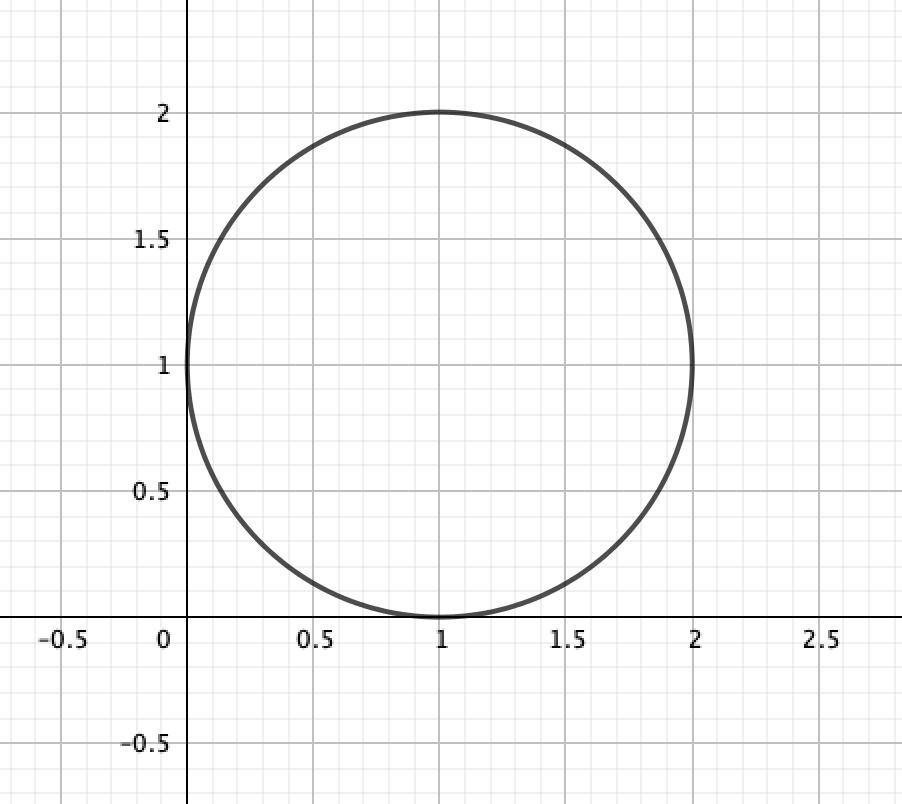
\includegraphics[width=0.5\linewidth]{./figures/e22f2.png}
  \caption{The curve $C$}
  \label{fig:e22f2}
\end{figure}

\paragraph{(b)} Find a parametric representation of the curve $C$.
If we let $\Vec{r}_0 (t) = \left( \cos t, \sin t, 0 \right) , 0 \leq t \leq 2 \pi$ denote the parametric representation of a circle with radius 1 with a centre at the origo we can find a parametric representation of our circle simply by adding the center point $\Vec{c}$ to this as:
\[ 
  \Vec{r}(t) = \Vec{c} + \Vec{r}_0(t) = \left( 1,1,0 \right) + \left( \cos t, \sin t, 0 \right) = \left( 1 + \cos t, 1 + \sin t, 0 \right), 0 \leq t \leq 2\pi
.\]



\subsection*{6.} Consider the curve $C$ given by the parametric representation
\[ 
\Vec{r}(t) = \left( \cos \left( t^2 \right) , 0, \sin \left( t^2 \right)  \right), 0 \leq t\leq \sqrt{2\pi}
.\]
Calculate the length of $C$.
\bigbreak
First we find the tangent as:
\[ 
\Vec{r}'(t) = \left( -2t \sin \left( t^2 \right) , 0, 2t \cos \left( t^2 \right)  \right) 
.\]
The scalar product is therefore:
\[ 
\Vec{r}'(t) \cdot \Vec{r}'(t) = \left( -2t \sin \left( t^2 \right), 0, 2t \cos \left( t^2 \right)  \right) \cdot \left( -2t \sin \left( t^2 \right) , 0, 2t \cos \left( t^2 \right)  \right) = 4t^2 \sin^2 \left( t^2 \right) + 0 + 4t^2 \cos^2 \left( t^2 \right) = 4t^2
.\]
The length can then be computed as:
\[ 
l \left( 0, \sqrt{2}\pi \right) = \int_{0}^{2\pi} \sqrt{ \Vec{r}'(t) \cdot \Vec{r}'(t)} \, \mathrm{d}t = \int_{0}^{\sqrt{2}\pi} 2t \, \mathrm{d}t = 2\pi
.\]

